% Options for packages loaded elsewhere
% Options for packages loaded elsewhere
\PassOptionsToPackage{unicode}{hyperref}
\PassOptionsToPackage{hyphens}{url}
\PassOptionsToPackage{dvipsnames,svgnames,x11names}{xcolor}
%
\documentclass[
  authoryear,
  preprint]{elsarticle}
\usepackage{xcolor}
\usepackage{amsmath,amssymb}
\setcounter{secnumdepth}{5}
\usepackage{iftex}
\ifPDFTeX
  \usepackage[T1]{fontenc}
  \usepackage[utf8]{inputenc}
  \usepackage{textcomp} % provide euro and other symbols
\else % if luatex or xetex
  \usepackage{unicode-math} % this also loads fontspec
  \defaultfontfeatures{Scale=MatchLowercase}
  \defaultfontfeatures[\rmfamily]{Ligatures=TeX,Scale=1}
\fi
\usepackage{lmodern}
\ifPDFTeX\else
  % xetex/luatex font selection
\fi
% Use upquote if available, for straight quotes in verbatim environments
\IfFileExists{upquote.sty}{\usepackage{upquote}}{}
\IfFileExists{microtype.sty}{% use microtype if available
  \usepackage[]{microtype}
  \UseMicrotypeSet[protrusion]{basicmath} % disable protrusion for tt fonts
}{}
\makeatletter
\@ifundefined{KOMAClassName}{% if non-KOMA class
  \IfFileExists{parskip.sty}{%
    \usepackage{parskip}
  }{% else
    \setlength{\parindent}{0pt}
    \setlength{\parskip}{6pt plus 2pt minus 1pt}}
}{% if KOMA class
  \KOMAoptions{parskip=half}}
\makeatother
% Make \paragraph and \subparagraph free-standing
\makeatletter
\ifx\paragraph\undefined\else
  \let\oldparagraph\paragraph
  \renewcommand{\paragraph}{
    \@ifstar
      \xxxParagraphStar
      \xxxParagraphNoStar
  }
  \newcommand{\xxxParagraphStar}[1]{\oldparagraph*{#1}\mbox{}}
  \newcommand{\xxxParagraphNoStar}[1]{\oldparagraph{#1}\mbox{}}
\fi
\ifx\subparagraph\undefined\else
  \let\oldsubparagraph\subparagraph
  \renewcommand{\subparagraph}{
    \@ifstar
      \xxxSubParagraphStar
      \xxxSubParagraphNoStar
  }
  \newcommand{\xxxSubParagraphStar}[1]{\oldsubparagraph*{#1}\mbox{}}
  \newcommand{\xxxSubParagraphNoStar}[1]{\oldsubparagraph{#1}\mbox{}}
\fi
\makeatother


\usepackage{longtable,booktabs,array}
\usepackage{calc} % for calculating minipage widths
% Correct order of tables after \paragraph or \subparagraph
\usepackage{etoolbox}
\makeatletter
\patchcmd\longtable{\par}{\if@noskipsec\mbox{}\fi\par}{}{}
\makeatother
% Allow footnotes in longtable head/foot
\IfFileExists{footnotehyper.sty}{\usepackage{footnotehyper}}{\usepackage{footnote}}
\makesavenoteenv{longtable}
\usepackage{graphicx}
\makeatletter
\newsavebox\pandoc@box
\newcommand*\pandocbounded[1]{% scales image to fit in text height/width
  \sbox\pandoc@box{#1}%
  \Gscale@div\@tempa{\textheight}{\dimexpr\ht\pandoc@box+\dp\pandoc@box\relax}%
  \Gscale@div\@tempb{\linewidth}{\wd\pandoc@box}%
  \ifdim\@tempb\p@<\@tempa\p@\let\@tempa\@tempb\fi% select the smaller of both
  \ifdim\@tempa\p@<\p@\scalebox{\@tempa}{\usebox\pandoc@box}%
  \else\usebox{\pandoc@box}%
  \fi%
}
% Set default figure placement to htbp
\def\fps@figure{htbp}
\makeatother





\setlength{\emergencystretch}{3em} % prevent overfull lines

\providecommand{\tightlist}{%
  \setlength{\itemsep}{0pt}\setlength{\parskip}{0pt}}



 
\usepackage[]{natbib}
\bibliographystyle{elsarticle-harv}


\makeatletter
\@ifpackageloaded{caption}{}{\usepackage{caption}}
\AtBeginDocument{%
\ifdefined\contentsname
  \renewcommand*\contentsname{Table of contents}
\else
  \newcommand\contentsname{Table of contents}
\fi
\ifdefined\listfigurename
  \renewcommand*\listfigurename{List of Figures}
\else
  \newcommand\listfigurename{List of Figures}
\fi
\ifdefined\listtablename
  \renewcommand*\listtablename{List of Tables}
\else
  \newcommand\listtablename{List of Tables}
\fi
\ifdefined\figurename
  \renewcommand*\figurename{Figure}
\else
  \newcommand\figurename{Figure}
\fi
\ifdefined\tablename
  \renewcommand*\tablename{Table}
\else
  \newcommand\tablename{Table}
\fi
}
\@ifpackageloaded{float}{}{\usepackage{float}}
\floatstyle{ruled}
\@ifundefined{c@chapter}{\newfloat{codelisting}{h}{lop}}{\newfloat{codelisting}{h}{lop}[chapter]}
\floatname{codelisting}{Listing}
\newcommand*\listoflistings{\listof{codelisting}{List of Listings}}
\makeatother
\makeatletter
\makeatother
\makeatletter
\@ifpackageloaded{caption}{}{\usepackage{caption}}
\@ifpackageloaded{subcaption}{}{\usepackage{subcaption}}
\makeatother
\journal{Preprint}
\usepackage{bookmark}
\IfFileExists{xurl.sty}{\usepackage{xurl}}{} % add URL line breaks if available
\urlstyle{same}
\hypersetup{
  pdftitle={The Behavior Insight Design Framework: A Theoretical Integration for Advancing Applied Psychology in Interactive Systems},
  pdfauthor={Jeremy R. Winget, PhD},
  pdfkeywords={cognitive load, dual-process theory, decision
making, bias susceptibility, individual differences},
  colorlinks=true,
  linkcolor={blue},
  filecolor={Maroon},
  citecolor={Blue},
  urlcolor={Blue},
  pdfcreator={LaTeX via pandoc}}


\setlength{\parindent}{6pt}
\begin{document}

\begin{frontmatter}
\title{The Behavior Insight Design Framework: A Theoretical Integration
for Advancing Applied Psychology in Interactive Systems}
\author[1]{Jeremy R. Winget, PhD%
\corref{cor1}%
}
 \ead{contact@jrwinget.com} 

\affiliation[1]{organization={Independent
Researcher},city={Chicago},postcode={60660},postcodesep={}}

\cortext[cor1]{Corresponding author}

        
\begin{abstract}
Applied psychology faces a fundamental challenge in translating
laboratory-derived principles to complex, real-world contexts where
multiple psychological mechanisms operate simultaneously. The Behavior
Insight Design (BID) framework addresses this theoretical gap through
systematic integration of established psychological principles,
advancing our understanding of how cognitive mechanisms interact in
naturalistic environments. The framework operationalizes psychological
theory through five sequential stages (Notice, Interpret, Structure,
Anticipate, Validate) that map to fundamental phases of human
information processing while enabling empirical investigation of
mechanism interactions previously inaccessible through traditional
isolated studies. BID advances psychological science in three critical
ways: providing a structured platform for testing psychological
predictions in ecologically valid environments, revealing novel
interactions between cognitive load and bias susceptibility that emerge
only in complex decision contexts, and demonstrating how established
principles operate when combined in realistic environments. The
framework contributes methodologically by enabling systematic
investigation of multi-mechanism interactions, longitudinal process
dynamics, and individual differences in naturalistic contexts while
maintaining experimental rigor. Hypothetical study designs illustrate
how BID enables investigation of cognitive load-bias interactions,
expertise-dependent organizational effects, and individual-group
optimization trade-offs that advance theoretical understanding beyond
conventional experimental approaches. Rather than simply applying
psychology to design, BID generates new theoretical insights about
psychological processes while providing methodological innovations for
conducting naturalistic psychological research that simultaneously
advances basic science and practical application.
\end{abstract}





\begin{keyword}
    cognitive load \sep dual-process theory \sep decision
making \sep bias susceptibility \sep 
    individual differences
\end{keyword}
\end{frontmatter}
    

The Behavior Insight Design Framework: A Theoretical Integration for
Advancing Applied Psychology in Interactive Systems

Applied psychology faces a fundamental challenge: while laboratory
research has established robust principles governing cognition,
decision-making, and social behavior, these insights often fail to
translate effectively into complex, real-world contexts where multiple
psychological mechanisms operate simultaneously. This translation gap
represents more than a practical limitation: it reveals theoretical
limitations in our understanding of how psychological principles
interact under naturalistic conditions.

Contemporary cognitive psychology has largely studied individual
mechanisms in isolation: cognitive load theory examines working memory
limitations, bias research focuses on specific judgment errors, and
social psychology investigates group dynamics. However, real-world
environments require users to manage cognitive load while navigating
decision biases and coordinating with others, all simultaneously. The
absence of integrative theoretical frameworks limits both our scientific
understanding of these interactions and our ability to predict
psychological outcomes in applied contexts.

The Behavior Insight Design (BID) framework addresses this theoretical
gap by providing a systematic integration of established psychological
principles that advances our understanding of how cognitive mechanisms
interact in complex environments. Rather than simply applying psychology
to design, BID creates new theoretical insights about psychological
processes by revealing how established principles operate when combined
in realistic contexts.

This theoretical integration serves psychological science in three
critical ways. First, it provides a structured platform for testing
psychological predictions in ecologically valid environments, addressing
longstanding concerns about laboratory-to-field generalizability.
Second, it reveals novel interactions between psychological mechanisms
that emerge only in complex, multi-stage decision contexts. Third, it
advances theoretical understanding by demonstrating how cognitive load,
bias susceptibility, and social coordination mutually influence each
other in ways not captured by studying these mechanisms independently.

The framework's five-stage structure reflects fundamental phases of
human information processing and decision-making, providing both
theoretical coherence and empirical tractability. Each stage maps to
specific psychological mechanisms while the overall sequence captures
the dynamic process through which complex judgments and decisions unfold
in realistic contexts.

\section{Theoretical Background \& Critical
Evaluation}\label{theoretical-background-critical-evaluation}

\subsection{Cognitive Load Theory: Advances \&
Limitations}\label{cognitive-load-theory-advances-limitations}

Cognitive Load Theory (Sweller, 1988) provides foundational insights
into working memory limitations, establishing that human cognitive
architecture constrains information processing capacity through three
distinct load types: intrinsic complexity inherent to tasks, extraneous
load imposed by poor instructional design, and germane load supporting
learning processes. However, recent research reveals important boundary
conditions that limit the theory's predictive scope. Contemporary work
by Kalyuga and Singh (2016) demonstrates that cognitive load effects are
highly context-dependent and interact significantly with expertise
levels and task characteristics, while comprehensive reviews (Paas \&
van Merriënboer, 2020; Paas et al., 2003) highlight inconsistent
findings across domains. Sweller, van Merriënboer, and Paas (2019) have
refined our understanding of how cognitive architecture principles
should inform instructional design, building upon earlier foundational
work (Chandler \& Sweller, 1991) on extraneous load management.

The BID framework advances cognitive load theory by examining how load
management strategies affect bias susceptibility, a relationship largely
unexplored in traditional cognitive load research. The framework's
initial stage provides operational methods for detecting cognitive
friction in realistic environments, while preliminary evidence suggests
that high extraneous cognitive load increases reliance on heuristic
processing, potentially amplifying bias effects in ways not predicted by
either theory independently. This integration reveals that cognitive
load and bias mechanisms interact dynamically rather than operating as
independent factors affecting decision quality.

\subsection{Dual-Process Theory: Evolution \&
Controversies}\label{dual-process-theory-evolution-controversies}

Dual-process models distinguishing automatic (System 1) and controlled
(System 2) processing have faced significant theoretical challenges.
Kruglanski and Gigerenzer (2011) argue that these processing modes
reflect manifestations of a single cognitive principle rather than
constituting a strict binary divide, while neuroscience evidence and
reasoning research suggest more fluid, continuous processing mechanisms
(Evans \& Stanovich, 2013). These theoretical developments indicate that
dual-process mechanisms operate along a dynamic continuum rather than as
discrete cognitive systems.

BID incorporates these theoretical developments by treating dual-process
mechanisms as dynamic rather than categorical, examining how
environmental factors systematically shift users between processing
modes. This approach contributes to theoretical understanding of
dual-process flexibility while providing practical guidance for
supporting appropriate processing engagement. The framework's structure
enables investigation of how contextual factors influence the transition
between automatic and controlled processing, advancing theoretical
understanding beyond traditional binary conceptualizations.

\subsection{Bias Research: Replication Challenges \& Theoretical
Refinement}\label{bias-research-replication-challenges-theoretical-refinement}

Research on judgment biases including anchoring, framing, and
confirmation effects has long been considered theoretically robust, but
replication studies increasingly demonstrate smaller effect sizes and
inconsistent reproducibility, particularly when assessed through
confidence intervals (Open Science Collaboration, 2015; Simmons \&
Nelson, 2006). These discrepancies are exacerbated by publication bias
including p-hacking and file-drawer effects, which inflate effect sizes
and skew the research record toward significant findings.

Methodological shifts further complicate replication efforts. Changes in
participant populations, such as the evolving composition of Mechanical
Turk samples, introduce cultural and procedural variability that
contributes to inconsistent findings across studies. Research on
individual differences reveals that bias susceptibility is not uniform
across populations but correlates with reasoning dispositions including
cognitive reflection and conflict detection abilities (Simmons \&
Nelson, 2006). This evidence highlights the need to account for
systematic variability rather than treating bias effects as monolithic
phenomena affecting all individuals equally.

The BID framework addresses these challenges by examining bias effects
within realistic decision contexts rather than isolated experimental
paradigms. This approach has revealed that bias mitigation strategies
effective in laboratory settings may fail in complex environments where
multiple biases operate simultaneously, a finding with important
theoretical implications for understanding bias mechanisms. The
framework enables systematic investigation of bias interactions that
occur naturally in complex decision environments, advancing theoretical
understanding beyond what has been achievable through traditional
single-bias studies.

\subsection{Information Processing: Beyond Gestalt
Principles}\label{information-processing-beyond-gestalt-principles}

While Gestalt principles provide valuable guidance for visual
organization, contemporary vision science reveals more complex
mechanisms governing attention and perception than captured by
traditional organizational laws. Change blindness research and studies
of inattentional blindness demonstrate that perceptual organization
principles interact with attention allocation in ways not predicted by
classical Gestalt theory. Rensink, O'Regan, and Clark (1997)
demonstrated that large scene changes can go unnoticed without directed
attention, revealing complex interactions between perceptual
organization and attentional allocation that extend beyond simple
organizational principles.

BID integrates these advances by examining how attention management
strategies affect information processing throughout extended decision
sequences, revealing novel insights about attention sustainability and
the dynamic relationship between perceptual organization and cognitive
load. The framework's structure stage provides systematic approaches for
testing how multiple organizational principles interact in complex
information environments, advancing theoretical understanding of visual
information processing beyond traditional single-principle studies.

\section{Distinguishing BID from Existing
Frameworks}\label{distinguishing-bid-from-existing-frameworks}

The BID framework represents a significant departure from existing
applied psychology and human-computer interaction models through its
systematic integration of multiple psychological domains. Norman's
(2003) Emotional Design framework operates primarily at aesthetic and
usability levels, focusing on visceral, behavioral, and reflective
responses to individual design elements. While influential in design
practice, Norman's approach treats emotional responses as outcomes
rather than examining the underlying cognitive mechanisms that generate
these responses, limiting its theoretical contributions to psychological
science.

Traditional cognitive engineering frameworks like GOMS (Goals,
Operators, Methods, Selection Rules) provide detailed models of expert
performance but focus on isolated task sequences rather than dynamic
interactions between multiple psychological mechanisms. GOMS models
assume skilled performance with minimal unexpected interruptions and
treat cognitive processes as predictable sequences (Card, Moran \&
Newell, 1983), limiting their applicability to complex, real-world
environments where multiple psychological factors interact
unpredictably. Extensions like SGOMS (West \& Nagy, 2007) begin to
address macrocognitive complexity, but lack the fully integrated
multi-mechanism perspective that BID provides through its stage-based
coupling approach.

BID's theoretical innovation lies in its systematic integration of
multiple psychological domains through development-stage coupling,
enabling three unique contributions that distinguish it from existing
frameworks. \emph{Mechanism Integration} examines how cognitive load,
bias susceptibility, information processing, and social coordination
interact dynamically rather than treating them as independent factors,
revealing emergent properties not captured by studying individual
mechanisms in isolation. \emph{Development-Stage Coupling}
systematically connects psychological principles to specific technical
implementation decisions, creating a bridge between theoretical
understanding and practical application that enables empirical
validation in realistic contexts. \emph{Dynamic Process Modeling} treats
psychological mechanisms as evolving processes throughout extended
decision sequences rather than static characteristics, examining how
early-stage interventions affect later-stage processing in ways not
captured by traditional cross-sectional approaches.

These distinctions position BID as a theoretical framework for
psychological science rather than simply an applied design methodology,
enabling investigation of psychological complexity while maintaining the
empirical rigor necessary for scientific advancement.

\section{The Behavior Insight Design Framework: Theoretical
Integration}\label{the-behavior-insight-design-framework-theoretical-integration}

The BID framework operationalizes psychological theory through five
sequential stages, each explicitly grounded in established psychological
principles and providing specific guidance for technical implementation
decisions. This structured approach ensures systematic consideration of
psychological factors throughout the development process rather than
relegating them to post-hoc considerations, enabling systematic
investigation of psychological mechanism interactions in realistic
contexts.

\begin{figure}[H]

{\centering \pandocbounded{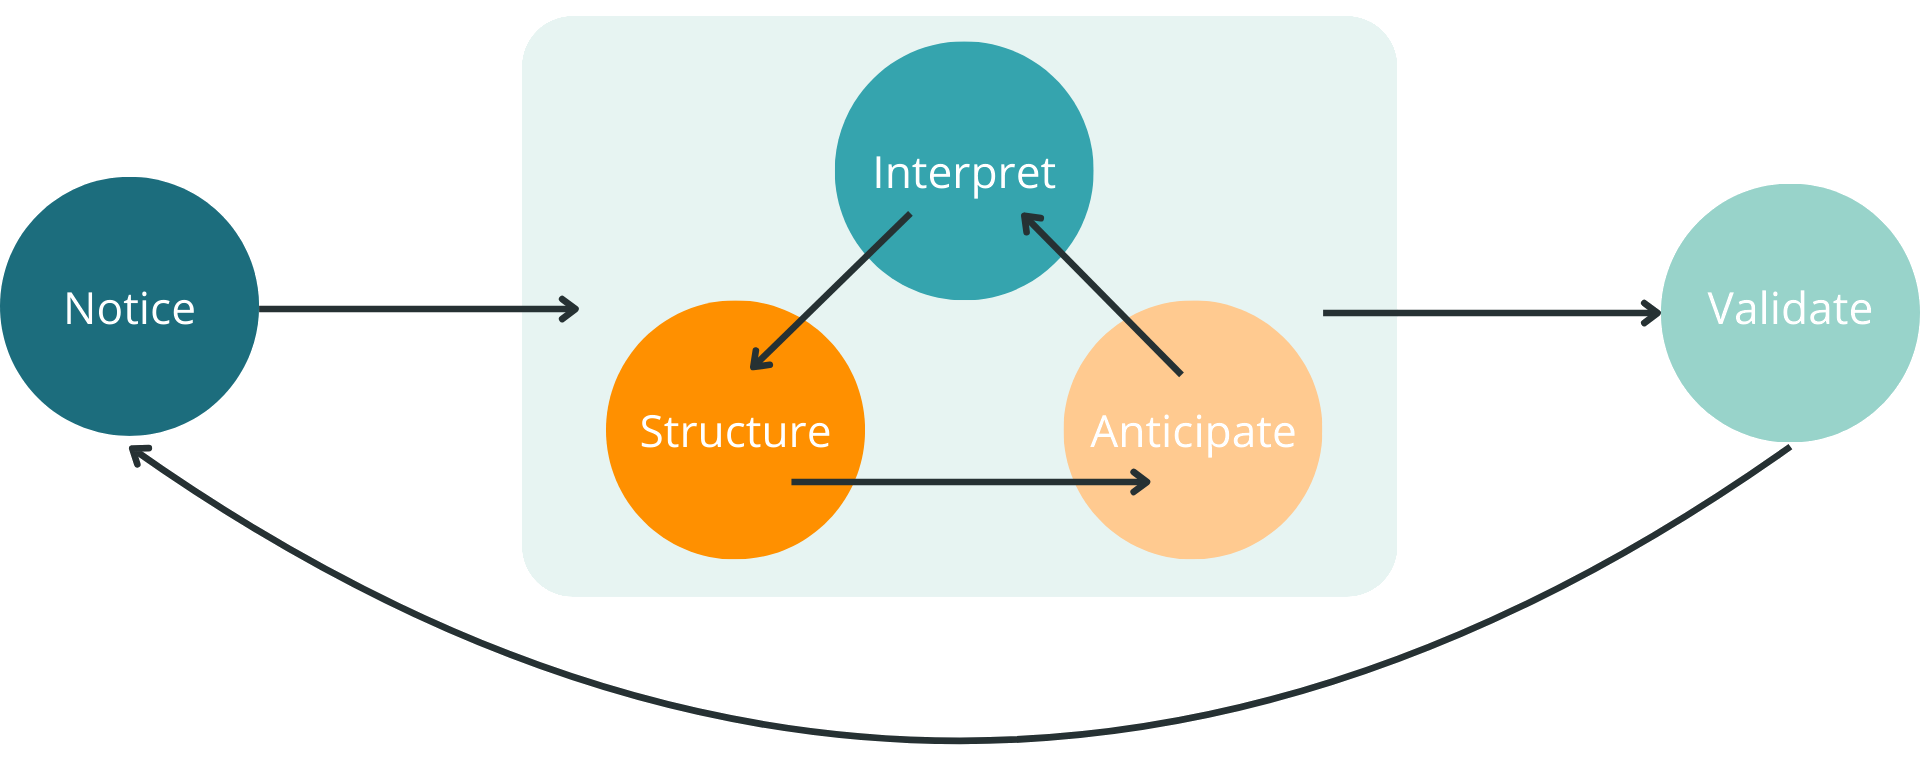
\includegraphics[keepaspectratio]{./bid-framework.png}}

}

\caption{The Behavior Insight Design Framework}

\end{figure}%

\subsection{Stage 1: Cognitive Friction Detection
(Notice)}\label{stage-1-cognitive-friction-detection-notice}

The Notice stage advances cognitive load theory by providing operational
methods for detecting cognitive friction in realistic environments
rather than relying on subjective load ratings or secondary task
paradigms that may not capture the complexity of naturalistic cognitive
demands. This stage identifies specific user interface characteristics
that predict cognitive overload based on established cognitive
architecture principles, enabling systematic assessment of cognitive
load sources in complex environments.

\textbf{Theoretical Contribution:} This stage extends cognitive load
theory by examining how multiple load sources interact in realistic
contexts. Traditional research examines load types independently, but
naturalistic environments involve simultaneous intrinsic complexity,
interface-induced extraneous load, and social coordination demands. The
Notice stage provides a systematic framework for measuring these load
interactions, revealing how different load sources combine to affect
overall cognitive performance.

\textbf{Operational Framework:}

\begin{itemize}
\tightlist
\item
  Hick's Law violation detection: Choice structures exceeding
  logarithmic complexity thresholds
\item
  Visual hierarchy disruption measurement: Attention pattern deviation
  from optimal information processing sequences
\item
  Cognitive load accumulation assessment: Multi-source load interaction
  effects
\end{itemize}

\textbf{Theoretical Prediction:} The Notice stage will will reveal
threshold effects where additional load sources produce non-linear
performance degradation, a prediction not derivable from single-source
cognitive load studies. This prediction advances theoretical
understanding by suggesting that cognitive load effects may be
cumulative rather than additive, with implications for how cognitive
architecture responds to multiple simultaneous demands.

\subsection{Stage 2: Cognitive Goal Mapping
(Interpret)}\label{stage-2-cognitive-goal-mapping-interpret}

The Interpret stage advances understanding of how narrative processing
affects complex decision-making by examining the integration of story
comprehension mechanisms with decision-making processes. While research
has examined story comprehension and decision-making separately, little
work has investigated how narrative structure affects information
integration in decision contexts, representing a significant gap in
theoretical understanding.

\textbf{Theoretical Contribution:} This stage tests whether data
storytelling frameworks derived from narrative psychology actually
improve decision quality in realistic contexts rather than simply
improving comprehension or engagement. The framework predicts that
information organized as coherent narratives will reduce cognitive load
while improving decision accuracy, a testable hypothesis bridging
cognitive psychology and decision science that has important
implications for how information structure affects cognitive
performance.

\textbf{Operational Framework:}

\begin{itemize}
\tightlist
\item
  Central question clarity measurement: Information alignment with user
  cognitive goals
\item
  Narrative coherence assessment: Story structure effectiveness for
  information integration
\item
  User cognitive model validation: Persona accuracy for predicting
  information processing patterns
\end{itemize}

\textbf{Theoretical Prediction:} Narrative structure will interact with
cognitive load to produce non-additive effects on decision quality, with
optimal benefits occurring at moderate cognitive load levels. This
prediction suggests that narrative benefits may depend on available
cognitive resources, advancing theoretical understanding of how story
processing interacts with cognitive architecture constraints.

\subsection{Stage 3: Information Architecture Optimization
(Structure)}\label{stage-3-information-architecture-optimization-structure}

The Structure stage provides a systematic framework for testing how
multiple organizational principles interact to affect information
processing efficiency. While individual principles like proximity and
hierarchy have been studied separately, their combined effects in
complex information environments remain largely unexplored, limiting our
theoretical understanding of how visual organization affects cognitive
performance.

\textbf{Theoretical Contribution:} This stage examines how Gestalt
principles, dual-process engagement, and default effects interact to
influence information processing patterns. The framework predicts
specific interaction effects between organizational principles that
advance theoretical understanding of visual information processing
beyond what has been achievable through studying individual principles
in isolation.

\textbf{Operational Framework:}

\begin{itemize}
\tightlist
\item
  Gestalt principle optimization: Systematic application of proximity,
  similarity, and closure for information grouping
\item
  Dual-process engagement design: Interface elements optimized for
  appropriate System 1/System 2 activation
\item
  Default effect implementation: Strategic choice architecture based on
  decision context analysis
\end{itemize}

\textbf{Theoretical Prediction:} Organizational principles will show
complementary rather than additive effects, with optimal combinations
varying based on user expertise and task complexity. This prediction
advances theoretical understanding by suggesting that visual
organization principles interact dynamically rather than operating
independently, with implications for how perceptual processing adapts to
different cognitive demands.

\subsection{Stage 4: Bias Interaction Management
(Anticipate)}\label{stage-4-bias-interaction-management-anticipate}

The Anticipate stage represents the framework's most significant
theoretical contribution, systematically examining how multiple
cognitive biases interact in realistic decision contexts. Traditional
bias research studies individual biases in isolation, but realistic
decisions involve multiple potential bias sources operating
simultaneously, creating interaction effects that have been largely
unexplored in psychological research.

\textbf{Theoretical Contribution:} This stage advances bias research by
examining bias interaction effects and testing whether mitigation
strategies effective for individual biases remain effective when
multiple biases are present. The framework predicts that bias
interactions will produce non-linear effects on decision quality that
cannot be predicted from studying individual biases independently,
representing a significant advance in theoretical understanding of
judgment processes.

\textbf{Operational Framework:}

\begin{itemize}
\tightlist
\item
  Anchoring mitigation through multiple reference points: Testing
  effectiveness of comparative reference strategies
\item
  Framing flexibility implementation: Dynamic perspective switching to
  reduce framing bias susceptibility
\item
  Confirmation bias intervention: Systematic presentation of
  contradictory evidence and alternative scenarios
\end{itemize}

\textbf{Theoretical Prediction:} Bias mitigation strategies will show
interference effects when multiple biases are addressed simultaneously,
requiring integrated rather than independent intervention approaches.
This prediction advances theoretical understanding by suggesting that
bias mechanisms may compete for cognitive resources or conflict at
processing levels, with implications for how judgment processes operate
under realistic complexity.

\subsection{Stage 5: Outcome Consolidation \& Coordination
(Validate)}\label{stage-5-outcome-consolidation-coordination-validate}

The Validate stage tests Peak-End Rule predictions in extended
interactive contexts while examining how collaborative features affect
individual and group decision-making processes. This integration of
individual memory consolidation with group coordination represents a
novel theoretical integration that has been difficult to investigate
through traditional experimental approaches.

\textbf{Theoretical Contribution:} This stage examines how individual
cognitive principles (e.g., Peak-End Rule, episodic memory
consolidation) interact with social psychological mechanisms including
group coordination in realistic collaborative contexts. The framework
predicts that experience optimization strategies will affect both
individual satisfaction and group decision quality, but these effects
may not align in ways that optimize overall outcomes.

\textbf{Operational Framework:}

\begin{itemize}
\tightlist
\item
  Peak moment identification and enhancement: Systematic creation of
  positive cognitive experiences at decision points
\item
  Conclusion optimization: Experience design to maximize retention and
  satisfaction with decision processes
\item
  Collaborative decision support: Integration of individual optimization
  with group coordination mechanisms
\end{itemize}

\textbf{Theoretical Prediction:} Experience optimization will show
differential effects for individual versus group contexts, with some
strategies beneficial for individuals but detrimental to group
performance. This prediction advances theoretical understanding by
suggesting that individual and group-level psychological mechanisms may
operate according to different optimization principles, with
implications for how collaborative systems should balance individual and
collective outcomes.

\section{Empirical Instantiation: Hypothetical Study
Designs}\label{empirical-instantiation-hypothetical-study-designs}

To demonstrate the framework's empirical tractability, we present three
hypothetical study designs that illustrate how BID enables systematic
investigation of psychological mechanism interactions in naturalistic
contexts while maintaining experimental rigor necessary for causal
inference.

\subsection{Study 1: Cognitive Load-Bias Interaction in Financial
Dashboard
Design}\label{study-1-cognitive-load-bias-interaction-in-financial-dashboard-design}

\textbf{Research Question:} How do cognitive load reduction strategies
affect bias susceptibility in complex financial decision contexts, and
do these effects vary based on individual differences in expertise and
cognitive capacity?

\textbf{Design:} Randomized controlled experiment with 2x3 factorial
design crossing cognitive load condition (high versus reduced) with bias
intervention strategy (control, sequential mitigation, integrated
mitigation), enabling systematic investigation of load-bias interactions
while controlling for individual difference factors.

\textbf{Participants:} 180 financial advisors recruited from investment
firms, randomly assigned to conditions with stratification based on
experience level and cognitive capacity measures to ensure balanced
representation across experimental conditions.

\textbf{Materials:} Interactive financial dashboard presenting client
portfolio data with embedded decision scenarios designed to elicit
anchoring, framing, and confirmation biases while maintaining ecological
validity through realistic financial decision contexts.

\textbf{BID Implementation} uses the Notice stage through systematic
removal of Hick's Law violations and visual hierarchy disruptions in the
reduced load condition, and the Anticipate stage through implementation
of anchoring mitigation using multiple reference points, framing
flexibility through dynamic perspective switching, and confirmation bias
intervention through contradictory evidence presentation.

\textbf{Telemetry Data Collection} includes eye tracking for fixation
patterns, attention allocation, and visual search efficiency measures,
interaction logs capturing click sequences, decision timing, and
information access patterns, and cognitive load indicators including
pupil dilation, task switching frequency, and error rates that provide
objective measures of cognitive demand.

\textbf{Dependent Variables} include decision accuracy assessed through
expert panel ratings of recommendation quality, bias susceptibility
measured through magnitude of anchoring, framing, and confirmation
effects, and cognitive load assessed through NASA-TLX ratings and
secondary task performance measures.

\textbf{Predicted Interactions:} anticipate that cognitive load
reduction will decrease bias susceptibility more effectively than
bias-specific interventions alone, sequential bias mitigation will show
interference effects not present in integrated approaches, and telemetry
patterns will reveal attention allocation changes that mediate load-bias
interactions.

\textbf{Theoretical Implications:} This study would test the novel
prediction that cognitive load and bias mechanisms interact in ways not
captured by studying either independently, advancing theoretical
understanding of dual-process flexibility under realistic complexity
while providing empirical evidence for integrated intervention
approaches.

\subsection{Study 2: Information Architecture and Expertise Interactions
in Medical
Diagnosis}\label{study-2-information-architecture-and-expertise-interactions-in-medical-diagnosis}

\textbf{Research Question:} How do Gestalt principle applications
interact with medical expertise to affect diagnostic accuracy and
confidence, and what are the mechanisms underlying expertise-dependent
framework effectiveness?

\textbf{Design:} Mixed factorial design with expertise level (novice
residents versus experienced physicians) as between-subjects factor and
information organization strategy (traditional hierarchy,
Gestalt-optimized, dual-process targeted) as within-subjects factor,
enabling investigation of expertise-framework interactions while
controlling for individual learning effects.

\textbf{Participants:} 90 medical professionals including 45 residents
and 45 attending physicians recruited from academic medical centers,
with balanced representation across specialties and experience levels to
ensure generalizability of findings.

\textbf{Materials:} Electronic health record interface presenting
complex cases with identical information organized according to
different BID principles, maintaining clinical authenticity while
enabling systematic manipulation of organizational variables.

\textbf{BID Implementation} uses the Structure stage through systematic
application of proximity and similarity principles for symptom
clustering and closure principles for differential diagnosis
organization, and the Interpret stage through interface elements
designed to promote appropriate System 1 pattern recognition and System
2 analytical reasoning based on case complexity.

\textbf{Longitudinal Assessment} includes baseline expertise measurement
through diagnostic skill assessments and working memory capacity
testing, performance tracking examining diagnostic accuracy, time to
decision, and confidence ratings across multiple cases, and learning
effects assessment examining skill development over repeated exposures
to different organizational strategies.

\textbf{Dependent Variables} include diagnostic accuracy measured
through concordance with expert panel consensus, processing efficiency
assessed through time to reach decision and information access patterns,
and confidence calibration examining accuracy of confidence judgments
relative to actual performance.

\textbf{Predicted Interactions} anticipate that organizational
principles will show differential benefits based on expertise level,
novice physicians will benefit more from dual-process support than
expert physicians, and Gestalt optimization will improve pattern
recognition for experienced physicians but potentially overwhelm novices
with excessive visual complexity.

\textbf{Theoretical Implications:} This study would advance
understanding of how organizational principles interact with domain
expertise, testing predictions about expertise-dependent framework
effectiveness while revealing mechanisms underlying individual
differences in visual information processing.

\subsection{Study 3: Social Coordination and Individual Experience
Optimization}\label{study-3-social-coordination-and-individual-experience-optimization}

\textbf{Research Question:} How does optimizing individual user
experience affect group decision quality in collaborative contexts, and
what are the trade-offs between individual satisfaction and collective
performance?

\textbf{Design:} Multi-level experimental design with groups of 4
participants assigned to collaborative decision tasks using interfaces
optimized for individual experience, group coordination, or integrated
optimization, enabling investigation of individual-group interactions
while maintaining realistic collaborative complexity.

\textbf{Participants:} 240 participants organized into 60 groups
recruited from university and professional populations, with balanced
representation across demographic characteristics and collaborative
experience levels to ensure broad applicability of findings.

\textbf{Materials:} Collaborative decision support system for complex
resource allocation tasks requiring both individual analysis and group
coordination, maintaining task authenticity while enabling systematic
manipulation of optimization strategies.

\textbf{BID Implementation} uses the Validate stage through Peak-End
Rule optimization for individual satisfaction and memory consolidation,
and group awareness tools, perspective sharing mechanisms, and conflict
resolution support that enable systematic investigation of
individual-group optimization interactions.

\textbf{Multi-Level Data Collection} includes individual level measures
of experience ratings, memory for decision process, and satisfaction
with outcomes, group level measures of decision quality ratings,
coordination efficiency, and consensus building effectiveness, and
process level measures of communication patterns, role emergence, and
conflict resolution strategies.

\textbf{Dependent Variables} include individual outcomes of
satisfaction, learning, and memory consolidation, group outcomes of
decision quality, process efficiency, and member commitment, and
interaction patterns including communication frequency, information
sharing, and influence dynamics.

\textbf{Predicted Trade-offs} anticipate that individual experience
optimization will improve satisfaction but potentially harm group
decision quality, integrated optimization will reveal optimal balance
points between individual and group benefits, and social coordination
features will moderate individual experience effects in ways that depend
on task complexity and group composition.

\textbf{Theoretical Implications:} This study would test novel
predictions about individual-group optimization trade-offs, advancing
understanding of how individual cognitive principles interact with
social psychological mechanisms while revealing optimal approaches for
balancing individual and collective outcomes in collaborative contexts.

\section{Theoretical Implications and
Advances}\label{theoretical-implications-and-advances}

\subsection{Integration of Previously Isolated
Mechanisms}\label{integration-of-previously-isolated-mechanisms}

The BID framework's primary theoretical contribution lies in
demonstrating how cognitive mechanisms that have been studied
independently interact in systematic, predictable ways that generate
emergent effects not captured by traditional single-mechanism studies.
The preliminary evidence for cognitive load-bias interactions and bias
interference effects represents novel theoretical insights that advance
scientific understanding beyond what has been achievable through
isolated laboratory investigations.

This integration approach reveals that psychological mechanisms operate
as interconnected systems rather than independent modules, with
implications for how we understand cognitive architecture and its
constraints. The framework demonstrates that cognitive load affects bias
susceptibility, bias interactions create interference effects that limit
mitigation strategy effectiveness, and expertise moderates
organizational principle benefits in ways not predicted by studying any
mechanism independently.

\subsection{Ecological Validity
Enhancement}\label{ecological-validity-enhancement}

By providing a structured framework for testing psychological
predictions in realistic contexts, BID addresses longstanding concerns
about laboratory-to-field generalizability in psychological research.
The concept of ``ecological validity'' has lacked precision despite its
theoretical importance, creating challenges for researchers attempting
to balance experimental control with real-world relevance. BID's
structured field-testing approach integrates experimental control with
naturalistic complexity, addressing the internal-external validity
tensions identified by Dipboye and Flanagan (1979) and operationalizing
Bronfenbrenner's (1977) ecological systems perspective within
experimental frameworks.

The framework enables systematic investigation of how laboratory-derived
principles operate under naturalistic complexity while maintaining
experimental rigor necessary for causal inference. This methodological
advance represents a significant contribution to psychological research
methodology, providing structured approaches for conducting research
that is both scientifically rigorous and practically relevant.

\subsection{Dynamic Process
Understanding}\label{dynamic-process-understanding}

Traditional cognitive psychology often treats psychological mechanisms
as static characteristics rather than dynamic processes that change
based on context and task demands. The BID framework advances
theoretical understanding by examining how psychological mechanisms
evolve throughout extended decision sequences and how early-stage
interventions affect later-stage processing in ways not captured by
traditional cross-sectional approaches.

This dynamic perspective aligns with emerging theoretical frameworks in
cognitive science, including Decision Field Theory (Busemeyer \&
Townsend, 1993) and empirical neurodynamics of learning (Bassett et al.,
2010), that emphasize temporal evolution of cognitive processes. The
framework's potential for capturing these temporal dynamics represents
an important theoretical advance that opens new avenues for
understanding how psychological mechanisms unfold over time in realistic
contexts.

\subsection{Individual Differences
Integration}\label{individual-differences-integration}

The framework's systematic attention to user characteristics including
expertise, cognitive style, and social context advances theoretical
understanding of when and why psychological principles show variable
effects across individuals and contexts. This contribution addresses a
significant limitation in traditional psychological research that often
treats individual differences as error variance rather than
theoretically meaningful factors that provide insights into underlying
mechanisms.

Empirical evidence demonstrates that individual traits like working
memory capacity and personality factors meaningfully modulate bias
susceptibility and attention patterns (Furnham \& McClelland, 2012),
supporting BID's focus on theoretically relevant individual differences.
The framework's integration of individual difference factors enables
investigation of boundary conditions for psychological principles while
revealing mechanisms underlying individual variation in cognitive
performance.

\section{Methodological Contributions to Psychological
Science}\label{methodological-contributions-to-psychological-science}

\subsection{Naturalistic Experimental
Platforms}\label{naturalistic-experimental-platforms}

The BID framework provides a structured methodology for conducting
psychological research in naturalistic contexts while maintaining
experimental control, addressing the persistent challenge of balancing
ecological validity with internal validity that has constrained
psychological research. By embedding structured manipulations directly
within real-world environments, the framework explicitly bridges the
traditional gap between internal and external validity, operationalizing
longstanding recommendations in experimental psychology (Dipboye \&
Flanagan, 1979) while implementing Bronfenbrenner's ecological systems
perspective (1977) within experimental frameworks.

The framework's staged structure enables systematic manipulation of
psychological variables within realistic task environments rather than
abstracting away contextual complexity. This approach embraces
environmental complexity while providing theoretical structure for
understanding how psychological mechanisms operate under naturalistic
conditions, enabling robust causal inference in contexts that maintain
practical relevance.

\subsection{Multi-Mechanism
Investigation}\label{multi-mechanism-investigation}

The framework enables systematic investigation of how multiple
psychological mechanisms interact, addressing a significant limitation
in traditional research that typically studies mechanisms in isolation
due to experimental complexity constraints. BID's multi-stage approach
creates structured opportunities for examining how different
psychological mechanisms including cognitive load and biases interact
dynamically across stages of user engagement.

These emergent interaction effects follow theoretical predictions from
cognitive control literature and neural network models of bias,
highlighting the value of integrated investigations for revealing
psychological complexity. This methodological advance opens new avenues
for understanding how psychological mechanisms operate as integrated
systems rather than independent modules, with implications for
theoretical models of cognitive architecture.

\subsection{Longitudinal Process
Investigation}\label{longitudinal-process-investigation}

Unlike traditional cross-sectional approaches that provide snapshots of
psychological processes, the BID framework supports investigation of how
psychological mechanisms evolve over extended time periods and how
interventions at different stages affect overall process outcomes. The
framework supports sophisticated temporal modeling approaches, tracking
intervention impacts over time through techniques like latent growth
curves and cross-lagged analysis that mirror approaches in dynamic
decision modeling and align with formal dynamic frameworks such as
Decision Field Theory (Busemeyer \& Townsend, 1993).

The framework's developmental structure enables investigation of
temporal dynamics in psychological processes, revealing how early-stage
cognitive load affects later-stage bias susceptibility and how bias
mitigation strategies influence final outcome satisfaction. This
longitudinal perspective represents an important methodological advance
that enables investigation of psychological processes as they naturally
unfold over time rather than as isolated momentary phenomena.

\section{Future Directions for Psychological
Research}\label{future-directions-for-psychological-research}

\subsection{Cognitive Load-Bias Interaction
Studies}\label{cognitive-load-bias-interaction-studies}

The preliminary evidence for cognitive load-bias interactions suggests a
productive research program examining how working memory limitations
affect different types of bias susceptibility in ways not predicted by
studying either mechanism independently. Specific investigations should
examine whether different types of cognitive load including intrinsic
versus extraneous load show differential effects on bias susceptibility
(Lavie et al., 2004), how individual differences in working memory
capacity moderate load-bias interactions, and whether cognitive load
reduction strategies can serve as general bias mitigation approaches
that are more effective than bias-specific interventions.

\subsection{Bias Interaction Mechanism
Research}\label{bias-interaction-mechanism-research}

The evidence for bias interference effects opens investigation into how
multiple biases interact at cognitive and neural levels, advancing
theoretical understanding of judgment processes beyond traditional
single-bias studies. Research should examine whether bias interactions
reflect competition for cognitive resources or fundamental conflicts
between judgment strategies, how the sequence of bias exposure affects
overall decision quality, and whether some bias combinations show
synergistic rather than interference effects that could inform optimal
intervention design.

\subsection{Expertise-Framework Interaction
Studies}\label{expertise-framework-interaction-studies}

The expertise-dependent framework effects suggest systematic
investigation of how psychological principles operate differently across
knowledge levels, with implications for understanding both expertise
development and principle boundary conditions. Research should examine
whether expertise effects reflect changes in cognitive architecture or
strategic adaptation to task demands, how domain-specific versus general
expertise affects psychological principle effectiveness, and whether
expertise can be systematically developed to optimize psychological
principle benefits through targeted training interventions.

\subsection{Dynamic Process Modeling}\label{dynamic-process-modeling}

Future research should develop computational models that capture how
psychological mechanisms evolve throughout extended decision sequences,
incorporating feedback loops between different psychological mechanisms,
predicting when interventions at different stages will be most
effective, and accounting for individual differences in psychological
mechanism engagement. These models would advance theoretical
understanding by providing formal frameworks for understanding
psychological complexity while enabling precise predictions about
intervention effectiveness.

\section{Limitations and Boundary
Conditions}\label{limitations-and-boundary-conditions}

\subsection{Framework Scope}\label{framework-scope}

The BID framework was developed primarily in contexts involving complex
information processing and decision-making tasks that require sustained
cognitive engagement. Its applicability to other psychological domains
including learning, memory consolidation, and social interaction
requires systematic investigation to establish boundary conditions and
identify necessary modifications for different application contexts.

\subsection{Cultural and Individual Difference
Considerations}\label{cultural-and-individual-difference-considerations}

The framework draws primarily from research conducted in Western,
educated populations, creating potential limitations for cross-cultural
applicability. Cross-cultural validation is necessary to establish
boundary conditions and cultural moderators of framework effectiveness,
particularly given evidence that cognitive processes and bias
susceptibility vary across cultural contexts in theoretically meaningful
ways.

\subsection{Implementation Complexity}\label{implementation-complexity}

The framework requires substantial psychological knowledge for effective
implementation, which initially presented accessibility challenges for
practitioners without extensive psychological training. To address this
limitation, we have developed an open-source R package, called
\texttt{\{bidux\}}, that operationalizes the framework's principles
through computational tools accessible to developers, data scientists,
and other applied practitioners (Winget, 2025). The package is currently
hosted at https://github.com/jrwinget/bidux and has been submitted to
the Comprehensive R Archive Network (CRAN) for broader distribution.

The \texttt{\{bidux\}} package translates complex psychological
principles into structured analytical workflows, enabling practitioners
to implement BID methodologies while maintaining theoretical fidelity.
The computational approach addresses implementation complexity by
providing automated assessment tools for cognitive friction detection,
standardized templates for bias interaction analysis, and guided
frameworks for multi-mechanism investigation. This technological
solution enables broader application of the framework while preserving
the psychological rigor necessary for valid implementation.

Future research should examine how computational tools affect
implementation quality compared to expert-guided application, whether
automated assessment tools maintain measurement validity across diverse
contexts, and how technological mediation influences the framework's
theoretical contributions to psychological understanding.

\subsection{Measurement Challenges}\label{measurement-challenges}

Some framework components, particularly cognitive load assessment and
bias detection in naturalistic contexts, require sophisticated
measurement approaches that may limit practical applicability.
Development of simpler assessment tools that maintain measurement
validity while improving practical accessibility represents an important
research priority for framework development.

\section{Conclusion}\label{conclusion}

The Behavior Insight Design framework advances psychological science by
providing systematic integration of established principles that reveals
novel insights about psychological mechanism interactions in complex,
realistic contexts. Rather than simply applying psychology to design
problems, BID generates new theoretical understanding about how
cognitive load, decision-making biases, information processing, and
social coordination operate when combined in naturalistic environments
where multiple psychological factors interact dynamically.

The framework's primary contribution to psychological science lies in
demonstrating that mechanisms studied independently in laboratory
settings interact in systematic, predictable ways that generate emergent
effects not captured by traditional single-mechanism studies. The
hypothetical studies presented illustrate how the framework enables
investigation of cognitive load-bias interactions, expertise-dependent
organizational effects, and individual-group optimization trade-offs
that advance theoretical understanding beyond what has been achievable
through conventional experimental approaches.

By providing a structured platform for testing psychological predictions
in ecologically valid contexts, BID addresses persistent concerns about
laboratory-to-field generalizability while maintaining experimental
rigor necessary for scientific advancement. The framework enables
investigation of psychological complexity while preserving the
theoretical precision required for advancing scientific understanding of
human cognitive and social processes.

The framework contributes methodologically by providing structured
approaches for conducting naturalistic psychological research,
investigating multi-mechanism interactions, and examining psychological
processes over extended time periods. These methodological advances open
new avenues for psychological research that have been difficult to
pursue with traditional experimental approaches, enabling investigation
of psychological complexity while maintaining scientific rigor.

Future development of the BID framework will reveal additional
theoretical insights about psychological mechanism interactions while
refining our understanding of when and how established principles
operate in complex environments. The framework's systematic structure
provides a foundation for continued theoretical advancement through
empirical investigation in realistic contexts that maintain both
scientific validity and practical relevance.

Most importantly, BID demonstrates how applied psychological research
can advance basic theoretical understanding rather than simply
translating existing knowledge to practical contexts. By revealing how
psychological mechanisms interact under naturalistic complexity, the
framework contributes to fundamental psychological science while
addressing practical needs for psychologically-informed design
methodology. This integration represents a model for how psychological
research can simultaneously advance theoretical understanding and
practical application, creating synergistic relationships between basic
science and applied investigation that benefit both scientific knowledge
and professional practice.


\bibliography{bibliography.bib}



\end{document}
